\section{Inside the transformer}
\label{sec:transformer}

\begin{sessioncard}
\textbf{Session 2.} \emph{Goal:} write down what a transformer computes, and see that its output is a sum of
contributions that we can inspect one at a time.
\emph{Experiments:} from which positions attention heads read (\cref{exp:attention}), after which layer the answer
appears (\cref{exp:lens}), and which components write the answer (\cref{exp:dla}).
\emph{Prerequisites:} session 1.
\end{sessioncard}

Almost all current language models are \emph{transformers} \citep{vaswani2017attention}. This session describes
the transformer used by GPT-2. We follow the description of \citet{elhage2021mathematical}, which is built around
the ``residual stream''. Most work in mechanistic interpretability uses this description.

\subsection{One vector per position}

Let the input consist of the tokens $t_1,\dots,t_n$, where each token is a number between $1$ and the size $V$
of the vocabulary. For every position $i$, the model stores a vector in $\R^d$ and updates it in every layer. This
vector is called the \emph{residual stream} at position $i$, or the \emph{stream} for short. We write
$x_i^{(\ell)}\in\R^d$ for its value at the input of layer $\ell$, where the layers are numbered $\ell=0,\dots,L-1$,
and $x_i^{(L)}$ for its final value. GPT-2 small has $L=12$ layers and $d=768$.

At the start, the stream is the sum of a vector for the token and a vector for the position,
\begin{equation}\label{eq:embed}
x_i^{(0)} \;=\; W_E[t_i] + W_{\mathrm{pos}}[i],
\end{equation}
where $W_E[t]\in\R^d$ is a learned vector for token $t$, called its \emph{embedding}, and
$W_{\mathrm{pos}}[i]\in\R^d$ is a learned vector for position $i$. At the end, the model computes the logits from
the final stream with one linear map, which we call the \emph{read-out}. For every token $t$ there is a learned
vector $W_U[t]\in\R^d$, called the \emph{unembedding} of $t$. The logit of token $t$ as the next token after
position $i$ is
\begin{equation}\label{eq:unembed}
\logit_i(t) \;=\; W_U[t]^\top\,\LN\big(x_i^{(L)}\big).
\end{equation}
Here $\LN$ is a normalisation, which we define next. Up to this normalisation, the logit of a token is large when
the final stream points in the direction of the unembedding of this token.

\paragraph{Layer normalisation.} Every component of the model reads the stream through the map
\begin{equation}\label{eq:ln}
\LN(x) \;=\; \frac{x-\mean(x)\,\one}{\scale(x)},\qquad
\mean(x)=\frac1d\,\one^\top x,\qquad
\scale(x)=\frac{1}{\sqrt d}\,\big\|x-\mean(x)\,\one\big\|,
\end{equation}
where $\one\in\R^d$ is the vector of ones. The map $\LN$ subtracts the average entry from every entry, and then
it rescales the vector to the length $\sqrt d$. This keeps the numbers in a range in which training works well. For
our analysis, $\LN$ is an inconvenience, because it is not linear: the factor $\scale(x)$ depends on $x$.
\Cref{prop:dla} below shows how we deal with this.

\subsection{What a layer adds}

Each layer contains two kinds of components: attention heads and an MLP. Both kinds read the stream and
\emph{add} their result to it (\cref{fig:residual}).

\begin{figure}[t]
\centering
\begin{tikzpicture}[>=Latex, font=\small,
  box/.style={draw=tutgrey, rounded corners=2pt, minimum height=6.5mm, inner sep=4pt, fill=#1},
  box/.default=white, add/.style={circle, draw=tutgrey, inner sep=0.5pt, fill=white}]
\draw[line width=1.8pt, tutblue] (0,0.35) -- (0,5.55);
\node[box=tutpaper] (emb) at (0,0) {embedding $W_E[t_i]+W_{\mathrm{pos}}[i]$};
\node (tok) at (0,-0.95) {token $t_i$};
\draw[->, tutgrey] (tok) -- (emb);
\node[add] (p1) at (0,2.35) {$+$};
\node[add] (p2) at (0,4.35) {$+$};
\node[box=tutblue!12] (att) at (4.2,1.55) {$\LN$, then the $H$ attention heads};
\node[box=tutred!12] (mlp) at (3.25,3.55) {$\LN$, then the MLP};
\draw[->, tutgrey] (0,1.55) -- (att.west);
\draw[->, tutgrey] (att.north) |- (p1);
\draw[->, tutgrey] (0,3.55) -- (mlp.west);
\draw[->, tutgrey] (mlp.north) |- (p2);
\node[align=left] (others) at (9.3,1.55) {streams $x_j^{(\ell)}$ of the\\ positions $j\le i$};
\draw[->, tutgrey] (others.west) -- (att.east);
\node[box=tutpaper] (un) at (0,5.9) {$\LN$, then unembedding $W_U$};
\node (out) at (0,6.85) {logits for the token after position $i$};
\draw[->, tutgrey] (un) -- (out);
\node[left] at (-0.1,1.0) {$x_i^{(\ell)}$};
\node[left] at (-0.1,3.0) {$\tilde x_i^{(\ell)}$};
\node[left] at (-0.1,5.0) {$x_i^{(\ell+1)}$};
\draw[decorate, decoration={brace, amplitude=5pt}, tutgrey] (-1.5,0.75) -- (-1.5,5.2)
  node[midway, left=6pt, align=right] {layer $\ell$,\\ repeated for\\ $\ell=0,\dots,L-1$};
\end{tikzpicture}
\caption{The residual stream at one position $i$ (thick blue line). Each component reads the stream through
$\LN$ and adds its output back. Only the attention heads see the streams of other positions.}
\label{fig:residual}
\end{figure}

\paragraph{Attention heads.} Attention heads are the only components that move information from one position to
another. Layer $\ell$ contains $H$ heads, numbered $h=0,\dots,H-1$. Each head has two learned matrices
$W_{QK},W_{OV}\in\R^{d\times d}$. Consider a position $i$, which we call the \emph{destination}, and a position
$j\le i$, which we call a \emph{source}. The head computes a score for every source. It turns the scores into
weights with a softmax over the sources, and it adds a weighted sum of vectors from the sources to the
destination:
\begin{align}
A^{\ell,h}_{ij} &\;=\; \frac{\exp\!\big(\LN(x_i^{(\ell)})^\top W_{QK}\,\LN(x_j^{(\ell)})\big)}
{\sum_{j'\le i}\exp\!\big(\LN(x_i^{(\ell)})^\top W_{QK}\,\LN(x_{j'}^{(\ell)})\big)},
\label{eq:pattern}\\
\head_i^{\ell,h} &\;=\; \sum_{j\le i}A^{\ell,h}_{ij}\;W_{OV}\,\LN(x_j^{(\ell)}) \;\in\R^d. \label{eq:headout}
\end{align}
The weights $A^{\ell,h}_{ij}$ are non-negative and sum to one over $j$. They are called the \emph{attention
pattern} of the head. The two matrices have different roles. The matrix $W_{QK}$ decides \emph{from where}
position $i$ reads: a source receives a large weight if the score between its stream and the stream of the
destination is large. The matrix $W_{OV}$ decides \emph{what} is written to position $i$ from each source. Because
of the restriction $j\le i$, a position never receives information from later positions. In GPT-2 small each layer
has $H=12$ heads. Each of the two matrices is stored as a product of a matrix with $64$ columns and a matrix with
$64$ rows, so its rank is at most $64$. We name a head by its layer and its index. For example, ``head 9.6'' is
head $h=6$ of layer $\ell=9$.

\paragraph{MLP.} After the heads, each layer contains an MLP (multilayer perceptron). The MLP applies two layers
similar to \eqref{eq:layer} to the stream at every position, separately for each position. Let
$\tilde x_i^{(\ell)}$ denote the stream after the heads of layer $\ell$ have added their output. Then
\begin{equation}\label{eq:mlp}
\mlp_i^{\ell} \;=\; W_{\mathrm{out}}\,\mathrm{GELU}\big(W_{\mathrm{in}}\,\LN(\tilde x_i^{(\ell)})+b_{\mathrm{in}}\big)+b_{\mathrm{out}} \;\in\R^d,
\end{equation}
with weight matrices $W_{\mathrm{in}}$, $W_{\mathrm{out}}$ and bias vectors $b_{\mathrm{in}}$, $b_{\mathrm{out}}$ that
belong to layer $\ell$. The function $\mathrm{GELU}$ is a smooth version of $\relu$, and it is applied to every
entry. The entries of the vector $\mathrm{GELU}(W_{\mathrm{in}}\,\LN(\tilde x_i^{(\ell)})+b_{\mathrm{in}})$ are
called the \emph{neurons} of the layer. GPT-2 small has $3072$ neurons in each layer.

\paragraph{Update rule.} Both kinds of components add their output to the stream:
\begin{equation}\label{eq:update}
\tilde x_i^{(\ell)} \;=\; x_i^{(\ell)}+\sum_{h=0}^{H-1}\head_i^{\ell,h},\qquad
x_i^{(\ell+1)} \;=\; \tilde x_i^{(\ell)}+\mlp_i^{\ell},\qquad \ell=0,\dots,L-1 .
\end{equation}
For simplicity, the formulas leave out some bias vectors and a constant factor in the scores. These details do
not affect anything in these notes. In GPT-2, the map $\LN$ also multiplies each entry by its own learned factor
and adds a learned vector. Both operations can be absorbed into the linear map that follows $\LN$, and the
software that we use does this when it loads the model.

\begin{intuition}
The residual stream works like a whiteboard at each position. Each head and each MLP reads what is written on
the whiteboard, computes something, and adds its result to the whiteboard. At the end, the answer is read from
the whiteboard by one linear map. Only the heads can copy information from the whiteboards of other positions.
\end{intuition}

\begin{experiment}[Where heads look]\label{exp:attention} \script{exp\_basics.py}
Attention patterns are the easiest quantities inside a transformer to look at. \Cref{fig:attention} shows
patterns of GPT-2 small on the prompts of the running example. The left panel shows the full pattern of head 4.11
on one prompt. Every destination puts almost all of its weight on the position directly before it. Averaged over
all positions and prompts, the weight on the previous position is $1.00$. A head with this pattern is called a
\emph{previous-token head}. The right panel shows the patterns of four heads at the last position, where the model
has to predict the name. Head 9.9 puts a weight of $0.79$ on the indirect object, $0.03$ on the first occurrence of
the subject and $0.04$ on the second occurrence. Heads 9.6 and 10.0 also put more weight on the indirect object than
on the subject. Their weights on the indirect object are $0.59$ and $0.31$, and their weights on each occurrence of
the subject are at most $0.12$. These patterns suggest a hypothesis: the three heads fetch the correct name and
write it into the last position. Head 10.7 also reads from the indirect object, with a weight of $0.82$.
\Cref{exp:dla} will show that this head has the opposite effect of the other three heads. The figure also shows
that head 10.0 puts almost half of its weight on the start token BOS. \Cref{ex:byhand}(c) asks why a head would do
this.
\end{experiment}

\begin{figure}[t]
\centering
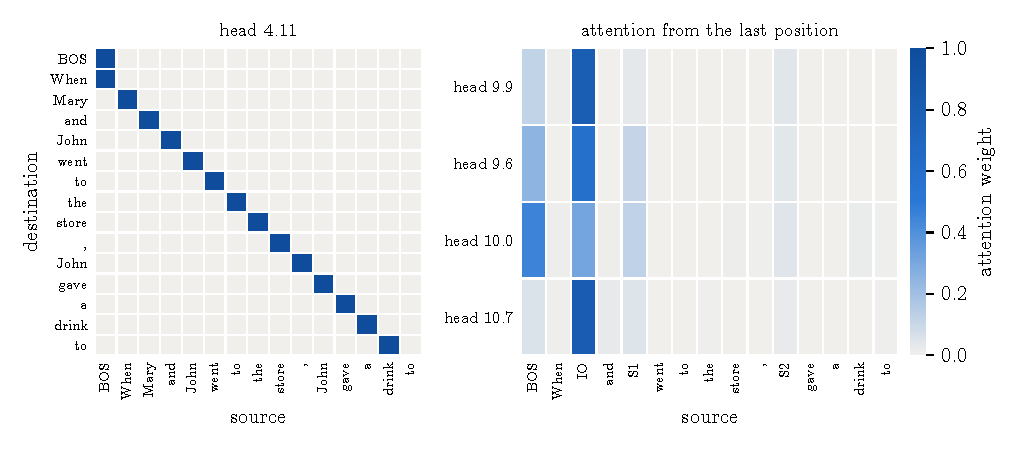
\includegraphics[width=0.92\textwidth]{figures/fig_attention.pdf}
\caption{Attention patterns in GPT-2 small (\cref{exp:attention}). Left: head 4.11 on one prompt. Each row is a
destination, and it shows how much weight this destination puts on each source. Right: four heads at the last position, averaged over
12 prompts. IO is the indirect object, S1 and S2 are the two occurrences of the subject.}
\label{fig:attention}
\end{figure}

\begin{caution}
An attention pattern shows \emph{from where} a head reads. It does not show \emph{what} the head writes, because
this is decided by $W_{OV}$. Moreover, in a late layer, the stream at a source position no longer describes only
the token at that position, because earlier heads have moved information from other positions there.
\end{caution}

\subsection{The output is a sum}
\label{sec:facts}

The update rule \eqref{eq:update} only adds vectors to the stream. This simple fact has a consequence on which
many methods of mechanistic interpretability are based.

\begin{proposition}[The final stream is a sum of component outputs]\label{prop:sum}
For every position $i$,
\begin{equation}\label{eq:sum}
x_i^{(L)} \;=\; W_E[t_i]+W_{\mathrm{pos}}[i]+\sum_{\ell=0}^{L-1}\Big(\sum_{h=0}^{H-1}\head_i^{\ell,h}+\mlp_i^{\ell}\Big).
\end{equation}
\end{proposition}
\begin{proof}
We write the final stream as a telescoping sum over the layers.
\begin{align*}
x_i^{(L)} &= x_i^{(0)}+\sum_{\ell=0}^{L-1}\big(x_i^{(\ell+1)}-x_i^{(\ell)}\big) && \by{telescoping sum}\\
&= x_i^{(0)}+\sum_{\ell=0}^{L-1}\Big(\sum_{h=0}^{H-1}\head_i^{\ell,h}+\mlp_i^{\ell}\Big) && \by{by \eqref{eq:update}}\\
&= W_E[t_i]+W_{\mathrm{pos}}[i]+\sum_{\ell=0}^{L-1}\Big(\sum_{h=0}^{H-1}\head_i^{\ell,h}+\mlp_i^{\ell}\Big). && \by{by \eqref{eq:embed}}\qedhere
\end{align*}
\end{proof}

\begin{proposition}[Each logit is a sum over components, given the final scale]\label{prop:dla}
Let $\mathcal G_i$ be the set of the $2+L(H+1)$ vectors on the right-hand side of \eqref{eq:sum}. We call them
the \emph{components} at position $i$. Then for every token $t$,
\begin{equation}\label{eq:dla}
\logit_i(t) \;=\; \sum_{g\in\mathcal G_i}\frac{W_U[t]^\top\big(g-\mean(g)\,\one\big)}{\scale\big(x_i^{(L)}\big)} .
\end{equation}
\end{proposition}
\begin{proof}
We insert the definition of $\LN$ and the sum of \cref{prop:sum} into the read-out.
\begin{align*}
\logit_i(t) &= W_U[t]^\top\,\LN\big(x_i^{(L)}\big) && \by{by \eqref{eq:unembed}}\\
&= \frac{W_U[t]^\top\big(x_i^{(L)}-\mean(x_i^{(L)})\,\one\big)}{\scale(x_i^{(L)})} && \by{by \eqref{eq:ln}}\\
&= \frac{W_U[t]^\top\big(\sum_{g\in\mathcal G_i}g-\mean\big(\sum_{g\in\mathcal G_i}g\big)\,\one\big)}{\scale(x_i^{(L)})} && \by{by \cref{prop:sum}}\\
&= \sum_{g\in\mathcal G_i}\frac{W_U[t]^\top\big(g-\mean(g)\,\one\big)}{\scale(x_i^{(L)})}. && \by{since $\mean$ is linear}\qedhere
\end{align*}
\end{proof}

The term of a component $g$ in the sum \eqref{eq:dla} is called the \emph{direct logit attribution} (DLA) of
$g$. It measures how much the vector that $g$ adds to the stream changes the logit directly. For the running
example, we apply \eqref{eq:dla} to the two names at the last position $n$ and take the difference:
\begin{equation}\label{eq:dla-ld}
\logit_n(\mathrm{IO})-\logit_n(\mathrm{S}) \;=\; \sum_{g\in\mathcal G_n}
\frac{\big(W_U[\mathrm{IO}]-W_U[\mathrm{S}]\big)^\top\big(g-\mean(g)\,\one\big)}{\scale\big(x_n^{(L)}\big)} .
\end{equation}
Two further facts follow directly from the definitions and will be used later.
\begin{itemize}
\item \textbf{Information moves between positions only through attention.} By \eqref{eq:mlp}, the output of an
MLP at position $i$ depends only on the stream at position $i$. The same holds for $\LN$ and for the read-out. So if
the stream at the last position contains information about an earlier token, some head must have moved this
information there.
\item \textbf{The coordinates of the stream have no special meaning.} Every component reads the stream through
a linear map after $\LN$, and it writes to the stream through a linear map. A rotation of $\R^d$ that leaves the
vector $\one$ fixed commutes with $\LN$. We can therefore rotate the stream by such a rotation and change all these
linear maps accordingly, and the model still computes the same function. So no coordinate of the stream, for
example coordinate number $17$, plays a special role. The neurons of an MLP are different, because $\mathrm{GELU}$
acts on each neuron separately.
\end{itemize}

\subsection{Two experiments based on the sum}

\begin{experiment}[The logit lens: when does the answer appear?]\label{exp:lens} \script{exp\_ioi.py}
By \eqref{eq:unembed}, the model computes its prediction from the final stream. The streams after every layer
are vectors in the same space $\R^d$. We can therefore apply the same read-out to the stream after $\ell$ layers
and compute $W_U[t]^\top\LN(x_n^{(\ell)})$ for $\ell=0,\dots,L$. This method is called the \emph{logit lens}
\citep{nostalgebraist2020logit}. Roughly speaking, it shows what the model would predict if it had to stop after
$\ell$ layers. \Cref{fig:lens} shows the logit lens on the running example. Up to $\ell=7$, the logit difference
under the lens stays between $-0.5$ and $0.5$. It becomes positive at $\ell=8$ and increases sharply at $\ell=10$,
that is, after layer 9 has been applied. On the first prompt, the most likely token under the lens is \tok{drink}
at $\ell=5$, \tok{the} at $\ell=8$, \tok{them} at $\ell=9$ and \tok{Mary} from $\ell=10$ onwards. So the decision
between the two names is written into the last position mainly by layer 9.

The figure shows a second effect. After 10 layers, the lens gives the correct name a probability of $0.998$, but
the complete model gives it only $0.48$. So layers 10 and 11 make the model \emph{less} confident.
\end{experiment}

\begin{figure}[t]
\centering
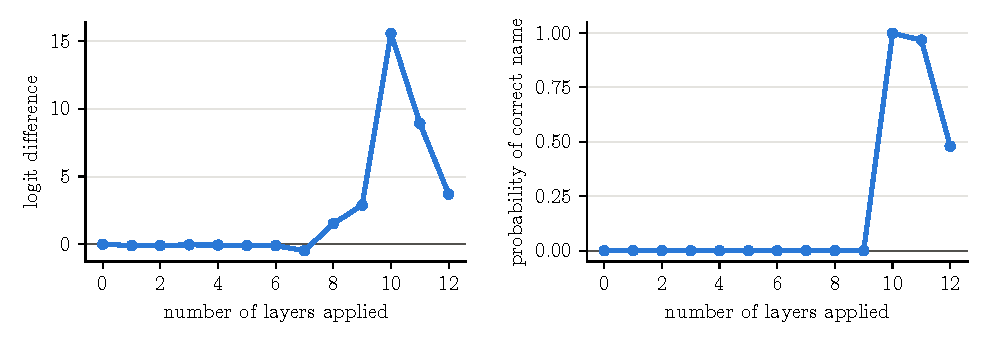
\includegraphics[width=0.82\textwidth]{figures/fig_logit_lens.pdf}
\caption{The logit lens on the IOI task (\cref{exp:lens}), at the last position, averaged over 12 prompts. Left:
logit difference between the correct and the repeated name. Right: probability of the correct name. The
horizontal axis is the number $\ell$ of layers that have been applied, so $\ell=12$ is the real output.}
\label{fig:lens}
\end{figure}

\begin{experiment}[Direct logit attribution: who writes the answer?]\label{exp:dla} \script{exp\_ioi.py}
We computed every term of the sum \eqref{eq:dla-ld}. The terms add up to $3.7031$, which is exactly the logit
difference measured at the output, as \cref{prop:dla} says. The 144 heads together contribute $3.45$, the 12 MLPs
contribute $0.25$, and the embeddings contribute less than $0.01$. \Cref{fig:dla} shows the contribution of every
head. Almost all heads contribute nearly nothing. Four heads clearly push towards the correct name: 9.9 ($+3.57$),
9.6 ($+1.10$), 10.6 ($+0.61$) and 10.0 ($+0.59$). Three of them are the heads that read from the indirect object in
\cref{exp:attention}. Two heads push \emph{against} the correct name: 10.7 ($-2.52$) and 11.10 ($-1.05$). These two
heads are in layers 10 and 11, and they explain why the model becomes less confident in these layers
(\cref{fig:lens}). \citet{wang2023interpretability} call 9.9, 9.6 and 10.0 \emph{name mover heads}, and they call
10.7 and 11.10 \emph{negative name mover heads}.
\end{experiment}

\begin{figure}[t]
\centering
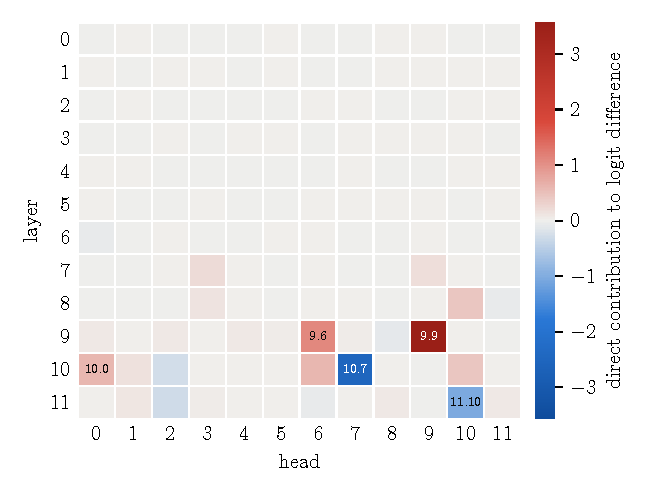
\includegraphics[width=0.5\textwidth]{figures/fig_dla_heads.pdf}
\caption{Direct logit attribution of every head of GPT-2 small to the logit difference of the IOI task
(\cref{exp:dla}), averaged over 12 prompts. Red heads push towards the correct name and blue heads push against
it.}
\label{fig:dla}
\end{figure}

\begin{caution}
Equation \eqref{eq:dla-ld} is an exact identity. Even so, the DLA of a component is not the same as the effect
of removing the component. A component also acts \emph{indirectly}: it changes what later components read. DLA
only measures the direct path from the component to the output. For example, head 9.9 might depend on a head in
layer 5 whose DLA is zero. Session 6 shows that this indeed happens in the running example.
\end{caution}

\begin{takeaways}
A transformer keeps one vector per position, the residual stream. Attention heads move information between
positions, MLPs process each position separately, and both add their output to the stream. The final stream is
therefore a sum of the outputs of all components, and each logit is a sum with one term per component. In the
running example, this decomposition shows that a few heads in layers 9 and 10 write most of the answer, and that
two heads in layers 10 and 11 work against it.
\end{takeaways}

\subsection*{Questions for the seminar}

\begin{exercise}[Attention by hand]\label{ex:byhand}
Consider one head with $d=2$ in a model without $\LN$. Let $W_{QK}=\begin{pmatrix}0&0\\2&0\end{pmatrix}$ and
$W_{OV}=\begin{pmatrix}0&0\\1&0\end{pmatrix}$, and let the stream be $x_1^{(\ell)}=(1,0)^\top$ at position $1$ and
$x_2^{(\ell)}=(0,1)^\top$ at position $2$. (a) Compute the attention pattern and the output of the head at the
destination $i=2$. (b) Do the same at the destination $i=1$. (c) The attention weights of a destination always sum to one, so a head cannot choose to read from no position
at all. How can a model still make a head write almost nothing at some destinations?
\end{exercise}

\begin{exercise}[A direction that nobody reads]\label{ex:ones}
Let $s\in\R$. Show that $\LN(x+s\,\one)=\LN(x)$. Conclude that replacing the stream $x_i^{(\ell)}$ by
$x_i^{(\ell)}+s\,\one$ at any single layer and position does not change any logit.
\end{exercise}

\begin{exercise}[Two heads with the same pattern]\label{ex:pattern}
Heads 9.9 and 10.7 both attend from the last position to the indirect object with a weight of about $0.8$, and
they have opposite effects on the output. (a) Which matrix is responsible for the difference? (b) Show that the
output \eqref{eq:headout} of a head has norm at most $\max_{j\le i}\|W_{OV}\LN(x_j^{(\ell)})\|$. (c) A head puts
the weight $0.9$ on a source whose vector $W_{OV}\LN(x_j^{(\ell)})$ has norm $0.1$, and the weight $0.1$ on a
source for which this norm is $10$. Which source dominates the output?
\end{exercise}

\begin{exercise}[What the logit difference hides]\label{ex:metric}
Suppose that some head raises the logits of all first names by the same amount at the last position of every IOI
prompt. (a) What is its contribution to \eqref{eq:dla-ld}? (b) Is this head irrelevant for the task? (c) Propose
a measure of performance under which its contribution becomes visible.
\end{exercise}

\begin{readinglist}
\item \citet{vaswani2017attention}, \emph{NeurIPS}. The original description of the architecture.
\item \citet{geva2022transformer}, \emph{EMNLP}. Describes the output of an MLP as a sum of updates to the stream
that are read through the unembedding, which is direct logit attribution for neurons.
\item \citet{kobayashi2020attention}, \emph{EMNLP}. Shows that the attention weight is only one of two factors in
what a head moves. The other is the norm of the transformed vector (\cref{ex:pattern}).
\item \citet{dar2023analyzing}, \emph{ACL}. Interprets the weights of a transformer directly, by expressing them
in the space of token embeddings.
\end{readinglist}
